%% Chapter 1
\chapter{Introduction}
\label{chap:intro}

\epigraph{No Battle Plan Survives Contact With the Enemy}{Helmuth von Moltke}

In order to meet the needs of an ever-growing user base,
software is expected to run in an increasing variety of deployment \emph{environments}. Generally, it is difficult to know everything that applications might come up against when deployed in such environments. As a consequence, it is perhaps not surprising that, no matter how well an application is tested before its release,
new bugs always seem to emerge after deployment.
Oracle estimates that 40\% of deployed applications
contain critical defects -- a situation that is compounded
by the fact that deployment
increases the cost to fix these flaws by 100 fold~\cite{OracleAppQuality}.

One reason for this outcome
is that differences between environments tend to
reveal previously undiscovered flaws.
These flaws emerge from
such factors as
operating system APIs changing across versions
~\cite{LinuxGlibcChanges, WinAPICompat, MuslDifferences},
or small variations in file systems exhibiting subtle but critical
differences~\cite{EXT4Layout, AppleHFS, WindowsNTFS}.
Even if the network and adapter are identical,
network behavior can still diverge from what is expected~\cite{vbox,
NMAPOSDifferences, VMWareNATFailure},
and these environmental differences greatly exacerbate
the chance that an application will function incorrectly when deployed.

These unforeseen bugs
complicate the work of 43\% of application developers who, according to a
recent survey conducted by ClusterHQ~\cite{ClusterHQSurvey},
spend between 10\% and 25\% of their time
debugging errors that only appear in production.
Numerous efforts have been made to reduce this burden.
One approach
is to hide environmental differences behind standard interfaces.
Unfortunately,
even specialized ``Write-Once, Run Anywhere'' environments
that attempt to hide these differences,
such as the Java Runtime Environment,
are not perfect,
leading them to be rechristened ``Write-Once, Debug Everywhere''~\cite{WODE}.
A more direct approach would be
to identify and fix deficiencies before deployment,
but history has shown that,
even if enormous effort is put forward,
it may be insufficient to uncover these bugs.
Microsoft employs thousands of engineers with nearly a
1:1 ratio of testers to developers~\cite{Page2009}.
Yet, a recent Windows Update released
in response to the Spectre Intel CPU vulnerability
resulted in machines with certain hardware configurations
being rendered unbootable~\cite{kb4056892}.

What is needed is a methodical way to record, preserve, and test against
specific features of any environment proven to have caused incorrect
behavior in applications.
By cataloging these features,
which we refer to as ``anomalies,'' and using them to systematically and reproducibly test other applications, we can predict behavior before deployment, saving time, developer effort, money, and most importantly the developer's reputation.
In this thesis we discuss the tools and techniques (illustrated in Figure~\ref{fig:overview}) we created in order to achieve this end.

\section{The SEA Technique}
The first major component of this work is a novel technique we refer to as Simulating Environmental Anomalies (SEA).
This technique is based on our finding that problematic features of an environment can often be identified in the results and side effects of the function calls, system calls, or other environmental interactions an application makes. When employing SEA,
an application under test is exposed
to the anomalies unique to a given environment
in such a way that its responses will indicate
potential for failures upon deployment. 
The technique allows users to define ``checkers''
to passively identify problems in application activity,
and ``mutators'' which modify activity streams so that they contain an anomaly.
This modified stream can then be replayed
in order to gauge an application's response.
These checkers and mutators may be shared between developers and applications providing 
easy and inexpensive way to learn from the mistakes of others.

We constructed
a proof-of-concept implementation of SEA called CrashSimulator. This tool a ``record-and-replay'' strategy to apply the technique on the system calls made by Linux applications.
By evaluating and modifying the parameters, return values, and side effects of these system calls we were able to expose
high-impact bugs in widely deployed applications.

\section{Pattern Observation Recognition and Transformation}
The second component is a new domain specific language that is specifically tailored toward making the expression of anomalies easier for developers.
The language,
known as PORT,
came about as a result of findings from a CrashSimulator user study that a general purpose programming language was insufficient for writing checkers and mutators.
The language is inspired by stream and event processing languages and offers a simple,
but powerful syntax for describing both opportunities to simulate an anomaly and what modifications must be made to a stream in order to do so.

One of our goals for PORT was to be able to extend the use of the SEA technique to other domains. To do so, we needed to show it could provide support for a variety of other ``activity representations'' such as XMLRPC requests, and USB traffic.
PORT allowed us to rewrite many of our existing CrashSimulator checkers and mutators in a simpler and more maintainable fashion.
Further, we demonstrated that we could write programs that can detect and simulate USB-based attacks and hardware bugs.


\begin{figure}[H]
  \center{}
  \fbox{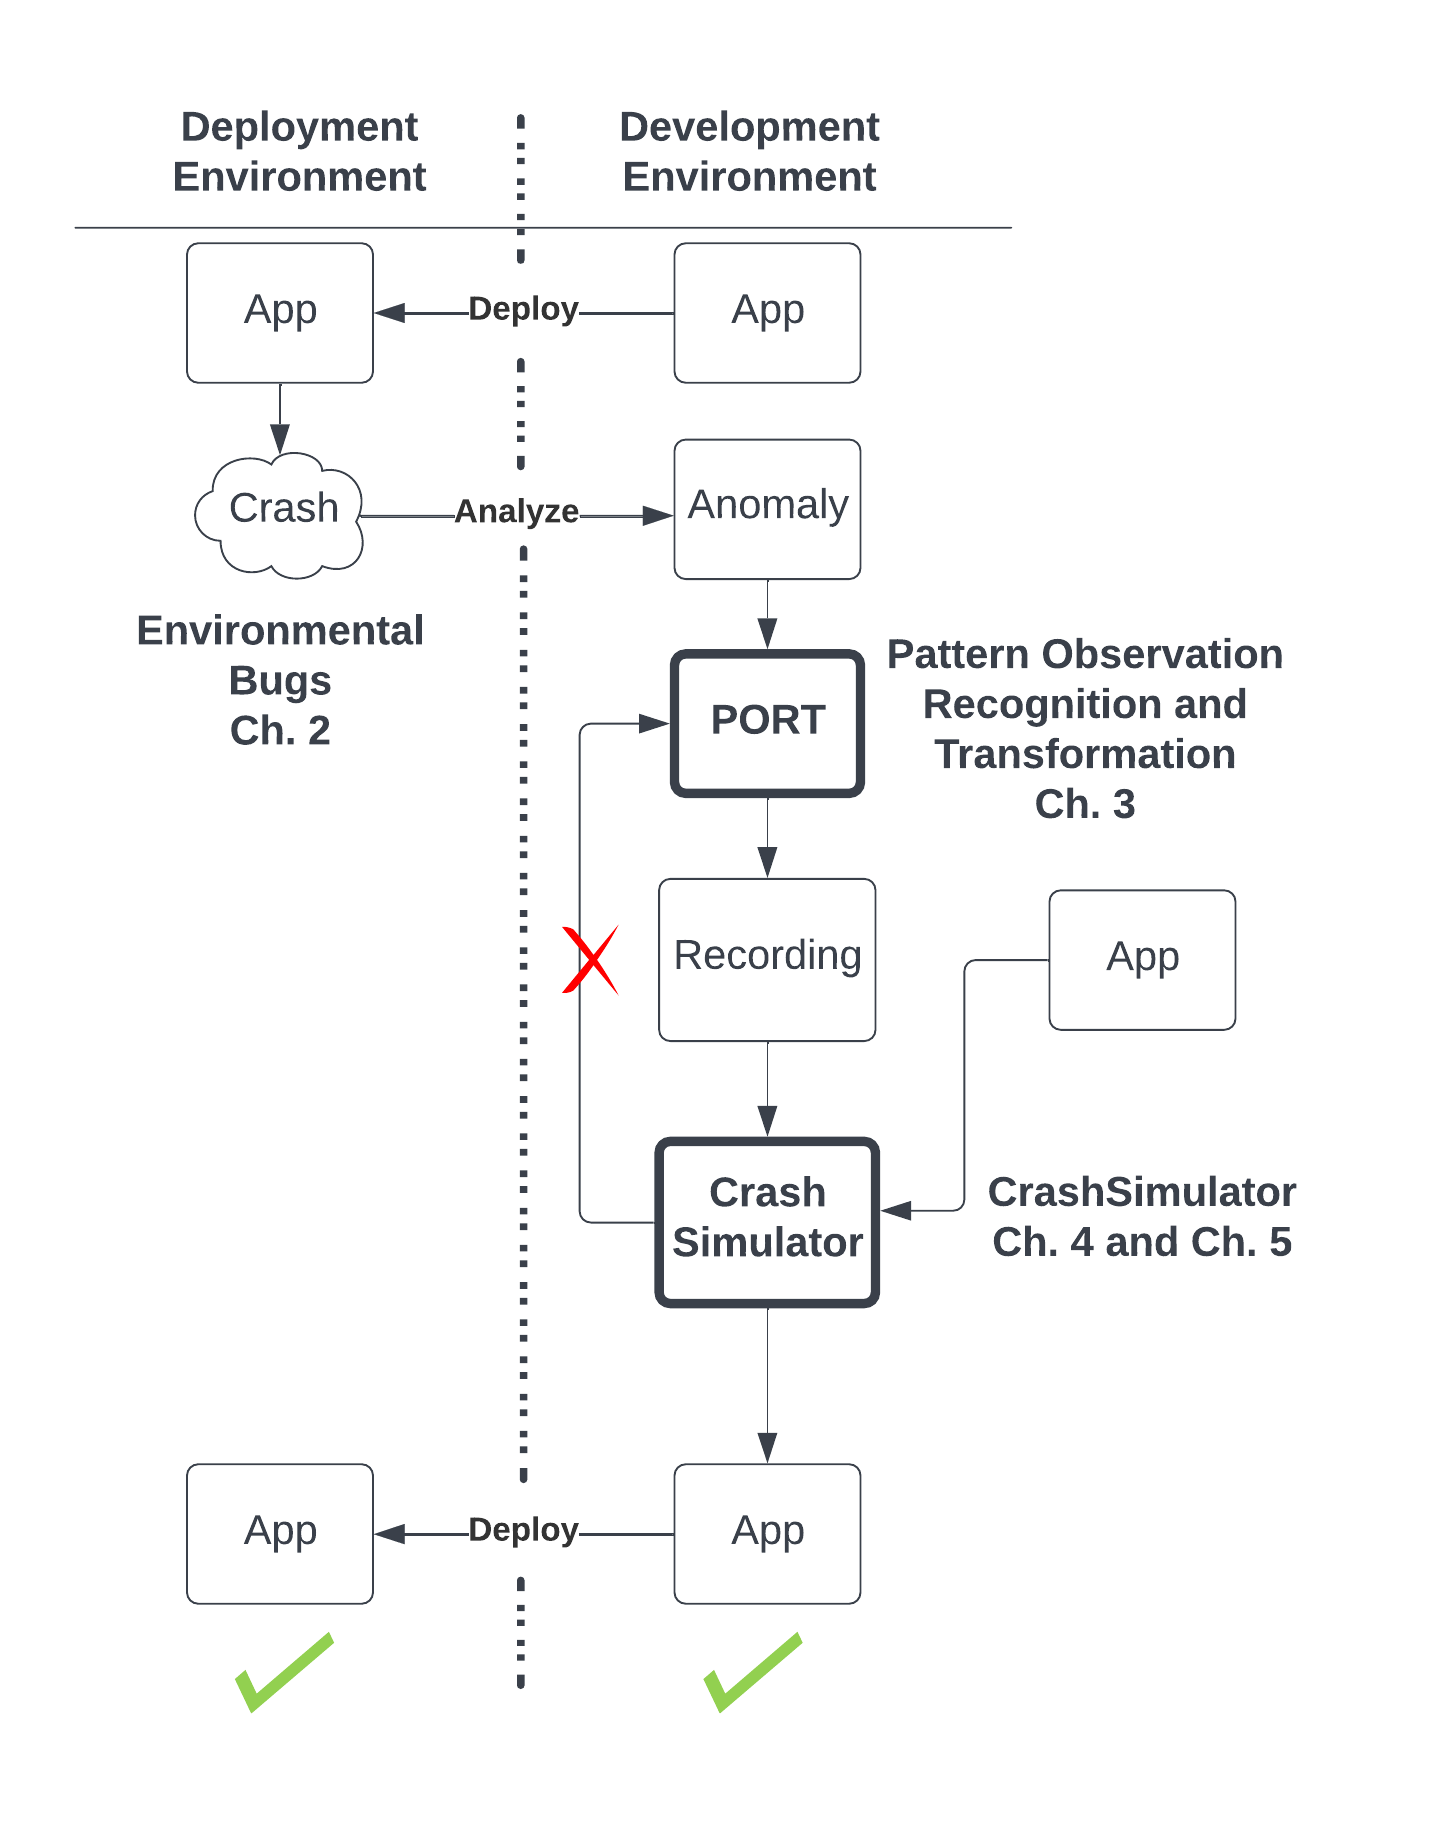
\includegraphics[scale=1.2]{chapter1/images/seaoverview}}
  \caption[Overview of Components]{This work discusses several tools and techniques that work together to help their users find environmental bugs.  This diagram offers an informal view of how they fit together.  Please refer to the chapters listed alongside the primary components for more detailed discussion about their operation.}
  \label{fig:overview}
\end{figure}

\section{A CrashSimulator User Study}
In order to determine how well CrashSimulator could be used by other developers we conducted a user study.
In this study our undergraduate and graduate student participants used the tool to hunt for bugs in applications of their choosing.
Once identified, they were asked to construct patches that fixed the bugs and submit them to upstream maintainers.
Our participants had success finding bugs and submitting patches but ran into resistance getting them accepted.
The reasons for this boil down to two deficiencies:
improper adherence to patch submission procedure and maintainers opinions that the identified failures are not bugs.
We discuss these outcomes, as well as direct feedback we received about CrashSimulator itself, in Chapter~\ref{chap:userstudy}.


\section{Organization of the thesis}
\label{sec:organization}
Chapter~\ref{chap:background}
presents an overview of environmental bugs, including where they
appear and how they can be detected.
The next chapter (Chapter~\ref{chap:sea})focuses on the development and testing of the SEA technique and the implementation and testing of CrashSimulator over system calls.
This is followed by the rationale for the second half of our work in  Chapter~\ref{chap:userstudy}. It presents results
from a user study conducted with CrashSimulator that
verified some of the tool's strengths and pointed out some weaknesses.
Chapter~\ref{chap:port}
is a direct response to usability issues raised in the previous chapter. It  discusses PORT,
our new domain specific language that addresses these weaknesses by making
it easier to find and modify interesting portions of streams of
application activity.
Chapter~\ref{chap:relatedwork}
compares our tools and techniques to earlier work in the areas of event stream processing languages, system call stream processing applications, API protocol mining, static analysis and more.
Finally,
Chapter~\ref{chap:conclusion} offers our closing thoughts and hopes for
the future of this work.
